\documentclass[12pt]{article}
\usepackage{amsmath, graphicx, caption}
\usepackage{amsthm}
\usepackage{amsfonts, xcolor, physics}
\usepackage{amssymb}
\usepackage{mathrsfs}
\usepackage[T1]{fontenc} % for \symbol{92} 
\usepackage{comment}


\addtolength{\oddsidemargin}{-1in}
\addtolength{\evensidemargin}{-1in}
\addtolength{\textwidth}{1.75in}
\addtolength{\topmargin}{-1in}
\addtolength{\textheight}{1.75in}
\newcommand{\contra}{$\rightarrow\leftarrow$}
\newcommand{\tb}{  \textbackslash  }
\newcommand{\bj}{\ \Longleftrightarrow \ }

%bailey meche
\begin{document}
%bailey meche
	\begin{center}
		Linear equations, inequalities, sets and functions, quadratics\\
        MACSS 33000 1 \\
		Due Tuesday, August 27 \\
        Bailey Meche
	\end{center}
 
\section{Simplify Expressions}
Simplify the following expressions as much as possible
\begin{enumerate}
    \item $(-x^4y^2)^2 = (-1)^2x^4y^2= x^8y^4$
    \item $9(3^0) = 9(1) = 9 $
    \item $(2a^2) (4a^4) = 8a^6$
    \item $\frac{x^4}{x^3}^3 = \left(\frac{x^4}{x^3}\right)^3= \left(x\right)^3 = x^3$
    \item $(-2)^{4-7} = (-2)^{-3} = \frac{1}{-2^3} = -\frac{1}{8}$
    \item $\left(\frac{1}{27b^3}\right)^{1/3}= \frac{1}{(27b^3)^{1/3}} = \frac{1}{3b}$
    \item $y^7y^6y^5y^4 = y^{7+6+5+4} = y^{22}$
    \item $\frac{2a/7b}{11b/5a} = \frac{2a}{7b} \cdot \frac{5a}{11b} = \frac{10a^2}{77b^2}$
    \item $(z^2)^4 = z^8$
\end{enumerate}

\section{Simplify a (more complex) expression}
Simplify the following expression
\begin{align*}
    & (a+b)^2 + (a-b)^2 + 2(a+b)(a-b) -3a^2
    \\ &= (a^2 + 2ab + b^2) + (a^2- 2ab +b^2) + (2a^2  - 2b^2) - 3a^2
    \\ &= a^2 
\end{align*}

\section{Graph sketching}
Let the functions $f(x)$ and $g(x)$ be defined for all $x \in \mathbb{R}$ by 
\begin{align*}
    &f(x) = \begin{cases}
    |x| & \text{if } x < 1 \\
    1 & \text{if } x \geq 1
\end{cases}, &  
g(x) = \begin{cases}
    x^2 & \text{if } x<2 \\
    4 & \text{if } x \geq 2
\end{cases}
\end{align*} 
\begin{enumerate}
    \item Sketch the graphs of:
    \item $y=f(x)$
    \item $y = g(x)$
    \item $y = f(g(x))$
    \item $y = g(f(x))$
\end{enumerate}
 
\begin{figure}[h!]
\centering
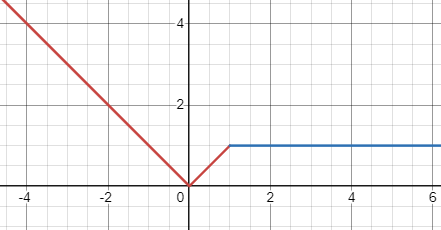
\includegraphics[height=6cm]{2.png}
\captionsetup{labelformat=empty}
\caption{2. $y = f(x)$}
\end{figure}


\begin{figure}[h!]
\centering
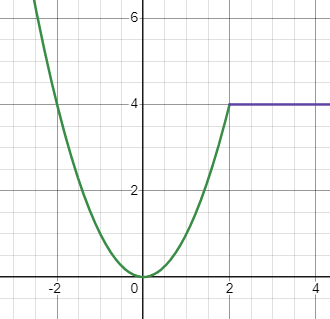
\includegraphics[height=6cm]{3.png}
\captionsetup{labelformat=empty}
\caption{3. $y = g(x)$}
\end{figure}


\begin{figure}[h!]
\centering
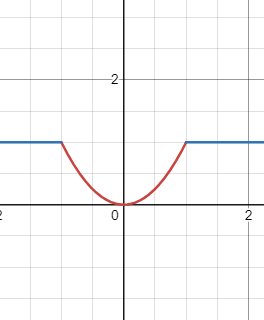
\includegraphics[height=6cm]{4.png}
\captionsetup{labelformat=empty}
\caption{4. $y = f(g(x))$}
\end{figure}


\begin{figure}[h!]
\centering
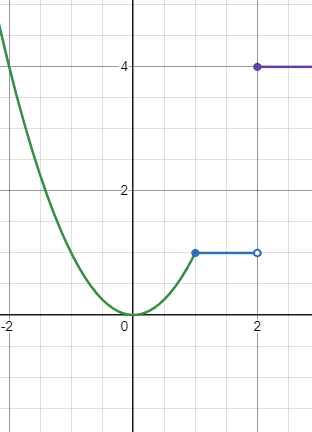
\includegraphics[height=6cm]{5.png}
\captionsetup{labelformat=empty}
\caption{5. $y = g(f(x))$}
\end{figure}


\section{Root finding}

Find the roots (solutions) to the following quadratic equations.
\begin{enumerate}
    \item $9x^2 - 3x - 12=0$
    \begin{align*}
        9x^2 - 3x - 12 &=0
        \\ 3(3x^2 - x- 4) &= 0
        \\ 3x^2 - x- 4 &= 0
        \\ 3x^2 - 4x + 3x - 4 &= 0
        \\ 3x(x +1) -4(x+1) &= 0
        \\ (3x-4)(x+1) &= 0 
        \\ x&= \frac{4}{3}, -1
    \end{align*}
    
    \item $x^2 - 2x -16 =0$
    \begin{align*}
        x^2 - 2x -16 &=0
        \\ x &= \frac{2 \pm \sqrt{4 - (4)(1)(-16)}}{2(1)}
        \\ x&=  \frac{2 \pm \sqrt{68}}{2}
        \\ x&=  \frac{2 \pm 2 \sqrt{17}}{2}
        \\ x&= 1+\sqrt{17}, 1-\sqrt{17}
    \end{align*}
    \item $6x^2 - 6x -6=0$
    \begin{align*}
        6x^2 - 6x -6 & =0
        \\ x^2 -x -1 &= 0
        \\ x&= \frac{1 \pm \sqrt{1 - 4(1)(-1)}}{2}
        \\ x&= \frac{1\pm \sqrt{5}}{2}
    \end{align*}
\end{enumerate}

\section{Systems of linear equations}
Solve the following systems of equations for their unknown values. If there is no solution, indicate as
such.
\begin{enumerate}
    \item Two unknowns 
    \begin{align*}
        3x - 2y &= 18
        \\ 5x + 10y &= -10
    \end{align*}
    Solution:
    \begin{align*}
        5(x+2y) &= -10
       \\ x + 2y &= -2
       \\ x &= -2y-2
       \\ 3(-2y-2) -2y&= 18
       \\ -6y -6 -2y &= 18
       \\ -8y &= 24
       \\ y&= -3
       \\ x&= -2(-3)-2 = 4
       \\ (x,y) &= (4,-3)
    \end{align*}

    \item Three unknowns 
    \begin{align*}
        5x - 2y + 3z &= 20
        \\ 2x - 4y - 3z &= -9
        \\ x + 6y -8z &= 21
    \end{align*}
    Solution: 
    \begin{align*}
        x + 6y -8z &= 21
        \\ x &= -6y + 8z +21
        \\ 2x - 4y - 3z &= -9
        \\ 2(-6y + 8z +21) - 4y - 3z &= -9
        \\ -12y + 16z + 42 -4y -3z &= -9
        \\ -16y + 13z &= -51
        \\ y &= \frac{13z +51}{16}
        \\ 5x - 2y + 3z &= 20
        \\ 5\left( -6\left(\frac{13z +51}{16}\right) + 8z +21 \right)-2\left(\frac{13z +51}{16}\right)+ 3z &= 20
        \\  -30\left(\frac{13z +51}{16}\right) +40z +105-2\left(\frac{13z +51}{16}\right)+ 3z &= 20
        \\ -32\left(\frac{13z +51}{16}\right) +43z &= -85
        \\ \frac{(-32)(13)z + (51)(-32)}{16} + \frac{(16)(43)z}{16} &= -85
        \\ \frac{272z + (51)(-32)}{16} &= -85
        \\ 17z + (51)(-2) &= -85
        \\ 17z &= 17
        \\ z&= 1
        \\ y &= \frac{13(1) + 51}{16} = 4
        \\ x&= -6(4) + 8(1) +21 = 5
        \\ (xyz) &= (5,4,1)
    \end{align*}

\item An animal shelter has a total of 350 animals comprised of cats, dogs, and rabbits. If the number of
rabbits is 5 less than one-half the number of cats, and there are 20 more cats than dogs, how many of
each animal are at the shelter?

Equation set: 
\begin{align*}
    c+d+r &= 350
    \\ r &= \frac{1}{2}c-5
    \\ c &= d+20
\end{align*}
Solution:
\begin{align*}
    (d+20) + d +\left( \frac{1}{2}(d+20) -5 \right) &= 350
    \\ \frac{5}{2}d +25 &= 350
    \\ d &= 130
    \\ c &= (130) + 20 = 150
    \\ r &= \frac{1}{2}(150) -5 = 70
    \\ (c,d,r) &= (150,130,70)
\end{align*}
\end{enumerate}


\section{Work with sets}
Using the setes
\begin{align*}
    A &= \{ 2,3,7,9,13,16\} 
    \\ B&= \{ x : 4\leq x \leq 8 \text{ and } x \text{ is an integer} \}
    \\ C &= \{ x : 2 < x < 25 \text{ and } x \text{ is prime}\}
    \\ D &= \{ 1,4,9,16,25,...\}
\end{align*}
Identify the following: 
\begin{enumerate}
    \item $ A \cup B$
    \item $(A \cup B) \cap C$
    \item $C \cap D$
\end{enumerate}
Solutions:
\begin{enumerate}
    \item $ A \cup B = \{ 2,3,9,13,16 \text{ and } x \in \mathbb{Z} | 4\leq x \leq 8 \} = \{ 2,3,4,5,6,7,8,9,13,16\}  $
    \item $(A \cup B) \cap C = \{ 2,3,4,5,6,7,8,9,13,16\} \cap  \{ x : 2 < x < 25 \text{ and } x \text{ is prime}\} = \{3,5,7,13\} $
    \item $C \cap D = \emptyset$
\end{enumerate}
\end{document}

%bailey meche